\documentclass[11pt]{article}

%%%%%%%%%%%%%%%%%%%%%%%%%%%%%%%%%%%%%%%%%%%%%%%%%%%%%%%%%%%%%%%
%                      Customize Header                       %
%%%%%%%%%%%%%%%%%%%%%%%%%%%%%%%%%%%%%%%%%%%%%%%%%%%%%%%%%%%%%%%

\newcommand{\assessmentTitle}{
CheckIt Assessment
}
\newcommand{\assessmentVersion}{
Version 1770005667924
}
\newcommand{\assessmentInstructions}{
Do not use any unapproved aids while taking this assessment.
Read each question carefully and be sure to show all work
in the space provided.
}

%%%%%%%%%%%%%%%%%%%%%%%%%%%%%%%%%%%%%%%%%%%%%%%%%%%%%%%%%%%%%%%
%%%%%%%%%%%%%%%%%%%%%%%%%%%%%%%%%%%%%%%%%%%%%%%%%%%%%%%%%%%%%%%



\usepackage{amsfonts,amssymb,amsmath,amsthm}
\setcounter{MaxMatrixCols}{50}
\usepackage{hyperref}
\let\oldhref\href\renewcommand{\href}[2]{\oldhref{#1}{#2}\footnote{\url{#1}}}
\usepackage[margin=1in,tmargin=2in,headheight=84pt]{geometry}
\usepackage{enumerate}
\usepackage{graphicx}
\usepackage{fancyhdr}
\usepackage{lastpage}
\pagestyle{fancy}
\fancyhf{}
\rhead{Name: \underline{\hspace{2.5in}}\\ID: \underline{\hspace{2.5in}}

\vspace{2.5em}}
\chead{\vspace{2.5em}

\fbox{\fbox{\parbox{6in}{\centering\assessmentInstructions}}}}
\lhead{\assessmentTitle \hspace{2em} \assessmentVersion

\vspace{2.5em}}
\rfoot{Page \thepage\ of \pageref{LastPage}}
\setlength{\headheight}{80pt}
\renewcommand{\headrulewidth}{0pt}


\begin{document}

\begin{enumerate}

% 

\item %%%%% SpaTeXt Commands %%%%%
\providecommand{\stxKnowl}{}\renewcommand{\stxKnowl}[1]{#1}
\providecommand{\stxOuttro}{}\renewcommand{\stxOuttro}[1]{#1}
\providecommand{\stxTitle}{}\renewcommand{\stxTitle}[1]{#1}
% Comment next line to show outtros
\renewcommand{\stxOuttro}[1]{}
%%%%%%%%%%%%%%%%%%%%%%%%%%%%
\stxKnowl{
Evaluate the function \(f(x) = 5 \, x^{2} + 8 \, x - 5\).

\begin{enumerate}
\item
\stxKnowl{
Find \(f(-8)\).

\stxOuttro{
SOLUTION

\(5(-8)^2 + 8(-8) + -5\)

\(\boxed{f(-8) = 251}\)

}
}

\item
\stxKnowl{
Find \(f(-x)\).

\stxOuttro{
SOLUTION

\(5(-x)^2 + 8(-x) + -5\)

\(\boxed{f(-x) = 5 \, x^{2} - 8 \, x - 5}\)

}
}

\item
\stxKnowl{
Find \(f(x + a)\).

\stxOuttro{
SOLUTION

\(5(x+a)^2 + 8(x+a) + -5\)

\(\boxed{f(x + a) = 5 \, a^{2} + 10 \, a x + 5 \, x^{2} + 8 \, a + 8 \, x - 5}\)

}
}

\end{enumerate}
}

\newpage

% 

\item %%%%% SpaTeXt Commands %%%%%
\providecommand{\stxKnowl}{}\renewcommand{\stxKnowl}[1]{#1}
\providecommand{\stxOuttro}{}\renewcommand{\stxOuttro}[1]{#1}
\providecommand{\stxTitle}{}\renewcommand{\stxTitle}[1]{#1}
% Comment next line to show outtros
\renewcommand{\stxOuttro}[1]{}
%%%%%%%%%%%%%%%%%%%%%%%%%%%%
\stxKnowl{
 Determine the number and type of solutions for the following equation: 

 \(3 \, x^{2} - 7 \, x - 1 = 6 \, x\) 

\stxOuttro{
SOLUTION

 \(3x^2 + (-13)x + -1 = 0\) 

 \(\Delta = (-13)^2 - 4(3)(-1)\) 

 \(\Delta = 181\) 

 \(\boxed{\text{ two solutions, unequal real roots }}\) 

}
}

\newpage

% 

\item %%%%% SpaTeXt Commands %%%%%
\providecommand{\stxKnowl}{}\renewcommand{\stxKnowl}[1]{#1}
\providecommand{\stxOuttro}{}\renewcommand{\stxOuttro}[1]{#1}
\providecommand{\stxTitle}{}\renewcommand{\stxTitle}[1]{#1}
% Comment next line to show outtros
\renewcommand{\stxOuttro}[1]{}
%%%%%%%%%%%%%%%%%%%%%%%%%%%%
\stxKnowl{
Solve for all solutions. Identify any extraneous solutions.

 \(x^{2} - 10 \, x + 28 = 0\) 

\stxOuttro{
SOLUTION

 \(x = \frac{-(-10) \pm \sqrt{(-10)^2 - 4(1)(28)}}{2(1)}\) 

 \(= \frac{10 \pm \sqrt{100 - 112}}{2}\) 

 \(= \frac{10 \pm \sqrt{-12}}{2}\) 

 \(= \frac{10 \pm 2i\sqrt{3}}{2}\) 

 \(= \frac{2(5 \pm i\sqrt{3})}{2}\) 

 \(\boxed{x = 5 \pm i\sqrt{3}}\) 

 (No extraneous solutions) 

}
}

\newpage

% 

\item %%%%% SpaTeXt Commands %%%%%
\providecommand{\stxKnowl}{}\renewcommand{\stxKnowl}[1]{#1}
\providecommand{\stxOuttro}{}\renewcommand{\stxOuttro}[1]{#1}
\providecommand{\stxTitle}{}\renewcommand{\stxTitle}[1]{#1}
% Comment next line to show outtros
\renewcommand{\stxOuttro}[1]{}
%%%%%%%%%%%%%%%%%%%%%%%%%%%%
\stxKnowl{
Solve for all solutions. Identify any extraneous solutions.

 \(\sqrt{x + 46} - 3 = 4\) 

\stxOuttro{
SOLUTION

 \(\sqrt{x + 46} = 7\) 

 \(x + 46 = 49\) 

 \(x = 49 - 46\) 

 \(\boxed{x = 3}\) 

 (No extraneous solutions) 

}
}

\newpage

% 

\item %%%%% SpaTeXt Commands %%%%%
\providecommand{\stxKnowl}{}\renewcommand{\stxKnowl}[1]{#1}
\providecommand{\stxOuttro}{}\renewcommand{\stxOuttro}[1]{#1}
\providecommand{\stxTitle}{}\renewcommand{\stxTitle}[1]{#1}
% Comment next line to show outtros
\renewcommand{\stxOuttro}[1]{}
%%%%%%%%%%%%%%%%%%%%%%%%%%%%
\stxKnowl{
 Solve for all solutions. Identify any extraneous solutions. 

 \(\displaystyle \frac{x}{x + 4} - \frac{20}{(x + 4)(x - 1)} = \frac{-3}{x - 1}\) 

\stxOuttro{
SOLUTION

 \(x(x - 1) - 20 = -3(x + 4)\) 

 \(x^{2} + 2 \, x - 8 = 0\) 

 \((x + 4)(x - 2) = 0\) 

 \(x = 2, \quad x = -4\) 

 \(x = -4 \implies \text{Extraneous}\) 

 \(\boxed{x = 2}\) 

}
}

\newpage

% 

\item %%%%% SpaTeXt Commands %%%%%
\providecommand{\stxKnowl}{}\renewcommand{\stxKnowl}[1]{#1}
\providecommand{\stxOuttro}{}\renewcommand{\stxOuttro}[1]{#1}
\providecommand{\stxTitle}{}\renewcommand{\stxTitle}[1]{#1}
% Comment next line to show outtros
\renewcommand{\stxOuttro}[1]{}
%%%%%%%%%%%%%%%%%%%%%%%%%%%%
\stxKnowl{
 Given that the function is one-to-one, find the inverse function \(f^{-1}(x)\). 

 \(f(x) = \sqrt[3]{x} - 1\) 

\stxOuttro{
SOLUTION

 \(y = f(x) = \sqrt[3]{x} - 1\) 

 \(x = \sqrt[3]{y} - 1\) 

 \(x + 1 = \sqrt[3]{y}\) 

 \((x + 1)^3 = y\) 

 \(y = (x + 1)^3\) 

 \(\boxed{ f^{-1}(x) = (x + 1)^3 }\) 

  

 \(= (x + 1)(x^2 + 2x + 1)\) 

 \(\boxed{ f^{-1}(x) = x^{3} + 3 \, x^{2} + 3 \, x + 1 }\) 

}
}

\newpage

% 

\item %%%%% SpaTeXt Commands %%%%%
\providecommand{\stxKnowl}{}\renewcommand{\stxKnowl}[1]{#1}
\providecommand{\stxOuttro}{}\renewcommand{\stxOuttro}[1]{#1}
\providecommand{\stxTitle}{}\renewcommand{\stxTitle}[1]{#1}
% Comment next line to show outtros
\renewcommand{\stxOuttro}[1]{}
%%%%%%%%%%%%%%%%%%%%%%%%%%%%
\stxKnowl{
Suppose a rocket carrying fireworks is launched from a hill 115 feet above a lake. The rocket's height \(h\) (in feet) above the lake at time \(t\) (in seconds) is given by

 \(h(t) = -16t^2 + 32t + 115\) 

\begin{enumerate}
\item
\stxKnowl{
When will the rocket reach its maximum height?

\stxOuttro{
SOLUTION

 \(t = \frac{-32}{2(-16)} = \frac{-32}{-32}\) 

 \(\boxed{t = 1 \text{ sec}}\) 

}
}

\item
\stxKnowl{
What is the maximum height the rocket will reach?

\stxOuttro{
SOLUTION

 \(h(1) = -16(1)^2 + 32(1) + 115\) 

 \(= -16 + 32 + 115\) 

 \(\boxed{h = 131 \text{ ft}}\) 

}
}

\item
\stxKnowl{
Interpret your results for the previous two questions in one or more complete sentences, including appropriate units.

\stxOuttro{
SOLUTION

The rocket will reach a maximum height of 131 ft 1 seconds after launch.

}
}

\end{enumerate}
}

\newpage

% 

\item %%%%% SpaTeXt Commands %%%%%
\providecommand{\stxKnowl}{}\renewcommand{\stxKnowl}[1]{#1}
\providecommand{\stxOuttro}{}\renewcommand{\stxOuttro}[1]{#1}
\providecommand{\stxTitle}{}\renewcommand{\stxTitle}[1]{#1}
% Comment next line to show outtros
\renewcommand{\stxOuttro}[1]{}
%%%%%%%%%%%%%%%%%%%%%%%%%%%%
\stxKnowl{
 Given \(f(x) = -2 \, x\) and \(g(x) = -3 \, x^{2} + 6\), find the following: 

\begin{enumerate}
\item
\stxKnowl{
\((f \circ g)(x)\)

\stxOuttro{
SOLUTION

 \(f(g(x)) = -2(-3 \, x^{2} + 6)\) 

 \(\boxed{ 6 \, x^{2} - 12 }\) 

ERROR 1: \(g(f(x))\)

 \(= -3(-2 \, x)^2 + 6\) 

 \(= -3(4 \, x^{2}) + 6\) 

 \(\boxed{ -12 \, x^{2} + 6 }\) 

ERROR 2: \(f(x) \cdot g(x)\)

 \(= (-2 \, x)(-3 \, x^{2} + 6)\) 

 \(\boxed{ 6 \, x^{3} - 12 \, x }\) 

}
}

\item
\stxKnowl{
\((f \circ f)(x)\)

\stxOuttro{
SOLUTION

 \(f(f(x)) = -2(-2 \, x)\) 

 \(\boxed{ 4 \, x }\) 

}
}

\end{enumerate}
}

\newpage

% 

\item %%%%% SpaTeXt Commands %%%%%
\providecommand{\stxKnowl}{}\renewcommand{\stxKnowl}[1]{#1}
\providecommand{\stxOuttro}{}\renewcommand{\stxOuttro}[1]{#1}
\providecommand{\stxTitle}{}\renewcommand{\stxTitle}[1]{#1}
% Comment next line to show outtros
\renewcommand{\stxOuttro}[1]{}
%%%%%%%%%%%%%%%%%%%%%%%%%%%%
\stxKnowl{
 Evaluate the difference quotient, \(\displaystyle{ \frac{f(x+h)-f(x)}{h}}\) , for \(f(x) = 2 \, x^{2} - 2\). 

\stxOuttro{
SOLUTION

 \(f(x+h) = 2(x+h)^2 - 2\) 

 \(= 2(x^2 + 2xh + h^2) - 2\) 

 \(= 2 \, h^{2} + 4 \, h x + 2 \, x^{2} - 2\) 

 \(\displaystyle{\frac{f(x+h)-f(x)}{h} = \frac{ (2 \, h^{2} + 4 \, h x + 2 \, x^{2} - 2) - (2 \, x^{2} - 2) }{h}}\) 

 \(=\displaystyle{ \frac{ 2 \, h^{2} + 4 \, h x }{h}}\) 

 \(= \displaystyle{ \frac{ h(2 \, h + 4 \, x) }{h}}\) 

 \(\boxed{ 2 \, h + 4 \, x }\) 

}
}

\newpage

% 

\item %%%%% SpaTeXt Commands %%%%%
\providecommand{\stxKnowl}{}\renewcommand{\stxKnowl}[1]{#1}
\providecommand{\stxOuttro}{}\renewcommand{\stxOuttro}[1]{#1}
\providecommand{\stxTitle}{}\renewcommand{\stxTitle}[1]{#1}
% Comment next line to show outtros
\renewcommand{\stxOuttro}[1]{}
%%%%%%%%%%%%%%%%%%%%%%%%%%%%
\stxKnowl{
 Consider the function: 

 \(f(x) = \frac{1}{4}(x - 6)^2 -9\) 

 Find the following properties: 

\begin{itemize}
\item
Vertex

\item
Axis of Symmetry

\item
\(x\)-intercepts

\item
\(y\)-intercept

\item
Domain

\item
Range

\end{itemize}
\stxOuttro{
SOLUTION

 \(\textbf{Direction: } \text{Opens Up}\) 

 \(\textbf{Vertex: } (6, -9)\) 

 \(\textbf{Axis of Symmetry: } x = 6\) 

 \(\textbf{x-intercepts:}\) 

 \(\frac{1}{4}(x - 6)^2 -9 = 0\) 

 \((x - 6)^2 = 36\) 

 \(x = 6 \pm 6\) 

 \(\boxed{ 0, 12 }\) 

 \(\textbf{y-intercept:}\) 

 \(= \frac{1}{4}(0 - 6)^2 -9\) 

 \(= \frac{1}{4}(36) -9\) 

 \(= 9 -9\) 

 \(\boxed{ 0 }\) 

 \(\textbf{Domain: } (-\infty, \infty)\) 

 \(\textbf{Range: } [-9, \infty)\) 

}
}

\newpage

% 

\item %%%%% SpaTeXt Commands %%%%%
\providecommand{\stxKnowl}{}\renewcommand{\stxKnowl}[1]{#1}
\providecommand{\stxOuttro}{}\renewcommand{\stxOuttro}[1]{#1}
\providecommand{\stxTitle}{}\renewcommand{\stxTitle}[1]{#1}
% Comment next line to show outtros
\renewcommand{\stxOuttro}[1]{}
%%%%%%%%%%%%%%%%%%%%%%%%%%%%
\stxKnowl{
 A quadratic function has the characteristics given below. Use the axis of symmetry to generate two additional points, then use all five points to graph the function. 

\begin{itemize}
\item
\(\text{Vertex: } (2, 2)\)

\item
\(x\text{-intercept: } 0\)

\item
\(y\text{-intercept: } 0\)

\end{itemize}
 \begin{tikzpicture}[scale=0.35] \draw[step=1cm, gray!40, very thin] (-10,-10) grid (10,10); \draw[thick, <->] (-10.5,0) -- (10.5,0); \draw[thick, <->] (0,-10.5) -- (0,10.5); \end{tikzpicture} 

\stxOuttro{
SOLUTION

 \begin{multicols}{2}  

\begin{itemize}
\item
\(\text{Vertex: } (2, 2)\)

\item
\(y\text{-intercept: } (0, 0)\)

\item
\(\text{Reflected } y\text{-int: } (4, 0)\)

\item
\(\text{Given Root: } (0, 0)\)

\item
\(\text{Reflected Root: } (4, 0)\)

\end{itemize}
 \columnbreak  

 \begin{tikzpicture}[scale=0.35] \draw[step=1cm, gray!40, very thin] (-10,-10) grid (10,10); \draw[thick, <->] (-10.5,0) -- (10.5,0); \draw[thick, <->] (0,-10.5) -- (0,10.5); \clip (-10,-10) rectangle (10,10); \draw[line width=1.5pt, blue!80!black, samples=100, domain=-10:10, <->] plot (\x, {-0.5*(\x - 2)^2 + 2}); \fill[blue] (2,2) circle (7pt); \fill[blue] (0,0) circle (7pt); \fill[blue] (4,0) circle (7pt); \fill[blue] (0,0) circle (7pt); \fill[blue] (4,0) circle (7pt); \end{tikzpicture} 

 \end{multicols} 

}
}

\newpage

% 

\item %%%%% SpaTeXt Commands %%%%%
\providecommand{\stxKnowl}{}\renewcommand{\stxKnowl}[1]{#1}
\providecommand{\stxOuttro}{}\renewcommand{\stxOuttro}[1]{#1}
\providecommand{\stxTitle}{}\renewcommand{\stxTitle}[1]{#1}
% Comment next line to show outtros
\renewcommand{\stxOuttro}[1]{}
%%%%%%%%%%%%%%%%%%%%%%%%%%%%
\stxKnowl{
 Use the table to identify the transformations described by \(g(x) = -f(-(x + 2)) - 3\). 

 Circle the option that applies and fill in the blanks as appropriate. Then apply these transformations to the graph of the function shown below. 

 \(\renewcommand{\arraystretch}{3} \begin{array}{|l|l|} \hline \textbf{Horizontal Transformations} & \textbf{Vertical Transformations} \\ \hline \text{Reflection: YES or NO} & \text{Reflection: YES or NO} \\ \hline \text{Dilation: \underline{\hspace{2cm}} times as wide} & \text{Dilation: \underline{\hspace{2cm}} times as tall} \\ \hline \text{Translation: \underline{\hspace{2cm}} units LEFT or RIGHT} & \text{Translation: \underline{\hspace{2cm}} units UP or DOWN} \\ \hline \end{array}\) 

 \noindent\makebox[\textwidth][c]{ \begin{minipage}{0.48\textwidth} \centering \begin{tikzpicture}[scale=0.39] \draw[step=1cm, gray!40, very thin] (-10,-10) grid (10,10); \draw[thick, <->] (-10.5,0) -- (10.5,0); \draw[thick, <->] (0,-10.5) -- (0,10.5); \draw[line width=1.5pt, black] (-2,1) -- (-1,2) -- (0,0) -- (1,4) -- (3,4);\fill[black] (-2,1) circle (5pt); \fill[black] (-1,2) circle (5pt); \fill[black] (0,0) circle (5pt); \fill[black] (1,4) circle (5pt); \fill[black] (3,4) circle (5pt); \end{tikzpicture} \end{minipage} \hfill \begin{minipage}{0.48\textwidth} \centering \begin{tikzpicture}[scale=0.39] \draw[step=1cm, gray!40, very thin] (-10,-10) grid (10,10); \draw[thick, <->] (-10.5,0) -- (10.5,0); \draw[thick, <->] (0,-10.5) -- (0,10.5); \end{tikzpicture} \end{minipage} } 

\stxOuttro{
SOLUTION



\begin{itemize}
\item
 \(\textbf{Horizontal: } \text{Reflection: YES, Dilation: 1, Shift: 2 units LEFT.}\) 

\item
 \(\textbf{Vertical: } \text{Reflection: YES, Dilation: 1, Shift: 3 units DOWN.}\) 

\end{itemize}


 \begin{tikzpicture}[scale=0.39] \draw[step=1cm, gray!40, very thin] (-10,-10) grid (10,10); \draw[thick, <->] (-10.5,0) -- (10.5,0); \draw[thick, <->] (0,-10.5) -- (0,10.5); \draw[line width=1.5pt, blue] (0,-4) -- (-1,-5) -- (-2,-3) -- (-3,-7) -- (-5,-7);\fill[blue] (0,-4) circle (5pt); \fill[blue] (-1,-5) circle (5pt); \fill[blue] (-2,-3) circle (5pt); \fill[blue] (-3,-7) circle (5pt); \fill[blue] (-5,-7) circle (5pt); \end{tikzpicture} 

}
}

\newpage

% 

\end{enumerate}

\end{document}